\chapter{Aspectos Estad\'isticos de la Homolog\'ia Persistente}\label{chap:Cap5}

Por s\'i sola, la homolog\'ia persistente no toma en cuenta la naturaleza estoc\'astica de los datos
y la variabilidad intrinseca de las cantidades topol\'ogicas que infieren.
Buscamos ahora un acercamiento esta\'distico a la homolog\'ia persistente,
considerando que los datos son generados de alguna distribuci\'on desconocida.
Comenzamos dando varos resultados de consistencia para la inferencia de la homolog\'ia persistente.

\section{Resultados de Consistencia para la Homolog\'ia Persistente}

Sup\'ongase que observamos $n$ puntos $\cpar{X_{1},\dots,X_{n}}$ en un espacio m\'etrico
$\cpar{M,\rho}$ obtenidas i. i. d. de una medida de probabilidad desconocida $\mu$ con
soporte compacto $\mathbb{X}_{\mu}$ la distancia de Gromov-Hausdorff nos permite comparar
$\mathbb{X}_{\mu}$ con otros espacios m\'etricos compactos no necesariamente encajados en $M$.
Definimos a continuaci\'on, $\hat{\mathbb{X}}$ un estimador de $\mathbb{X}_{\mu}$
como una funci\'on de $X_{1},\dots,X_{n}$ que toma valores en el conjunto de espacios m\'etricos compactos.

Sean $\mathrm{Filt}\cpar{\mathbb{X}_{\mu}}$ y $\mathrm{Filt}\cpar{\hat{\mathbb{X}}}$
dos filtraciones definidas en $\mathbb{X}_{\mu}$ y $\hat{\mathbb{X}}$.
Con el teorema \ref{teo:4.9} hemos visto que una estrategia natural
para estimar la homologi\'ia persistente de $\mathrm{Filt}\cpar{\mathbb{X}_{\mu}}$
consiste en estimar el soporte de $\hat{\mathbb{X}}$.
N\'otese que en algunos casos, el espacio $M$ puede ser desconocido
y las observaciones $X_{1},\dots,X_{n}$ solo se conocen mediante de sus distancias por pares
$\rho\cpar{X_{i}, X_{j}}$, $i$, $j = 1,\dots,n$.
La distancia de Gromov-Hausforff nos permite considerar el conjunto de observaciones
como un espacio m\'etrico abstracto de cardinalidad $n$,
independietemente de la manera en la que esta encajado en $M$.
Esta estructura general incluye el acercamiento m\'as est\'andar
que consiste en estamar el soporte con respecto a la distancia de Hausdorff
restringiendo los valores de $\hat{\mathbb{X}}$ a los conjuntos compactos en $M$.

El conjunto finito $\mathbb{X}_{n}:=\cllav{X_{1},\dots,X_{2}}$
es un estimador natural para el soporte de $\mathbb{X}_{\mu}$.
En muchos de los contextos que veremos a continuaci\'on,
$\mathbb{X}_{\mu}$ muestra tasas de convergencia \'optimas
con respecto a la ditancia de Hausdorff.
Para algunas constantes $a,b>0$, decimos que $\mu$ satisface el supuesto
$\cpar{a,b}$-est\'andar si para cualquier $x\in\mathbb{X}_{\mu}$ y cualquer $r>0$,
\begin{equation}
    \mu\cpar{B\cpar{x,r}}\geq\min\cpar{ar^{b},1}.
\end{equation}

Este supuesto es ampliamente usado en la literatura de la estimaci\'on de conjuntos
bajo la distancia de Hausdorff
(Cuevas y Rodriguez-Casal, 2004\cite{CuevasRodriguezCasal2004};
Singh et al., 2009\cite{Singh2009}).
Bajo este supuesto, puede deducirse que la tasa de convergencia de
$\mathrm{dgm}\cpar{\mathrm{Filt}\cpar{\mathbb{X}_{n}}}$ a
$\mathrm{dgm}\cpar{\mathrm{Filt}\cpar{\mathbb{X}_{\mu}}}$
para la m\'etrica de cuello de botella es acotada superiormente por
$O\cpar{\frac{\log n}{n}}^{1/b}$. M\'as precisamente, esta tasa
acota superiormente la tasa de convergencia minimax sobre el conjunta de medidas
de probabilidad en el espacio m\'etrico $\cpar{M, \rho}$ satisfaciendo el supuesto
$\cpar{a,b}$-est\'andar en $M$.

\begin{teorema}
    Chazal et al. (2014)\cite{Chazal2014b} para algunas constantes positivas, $a$ y $b$, sea
    \begin{equation*}
        \mathcal{P}:=\cllav{\mu \text{ en } M |
        \mathbb{X}_{\mu}\text{ es compacto y }\forall x\in\mathbb{X}_{\mu},\forall r>0,\hspace{4pt}
        \mu\cpar{B\cpar{x,r}}\geq\min\cpar{1,ar^{b}}}
    \end{equation*}
    Entonces, se tiene que
    \begin{equation*}
        \sup_{\mu\in\mathcal{P}}\mathbb{E}\ccorch{
        \mathrm{d}_{\mathrm{b}}\cpar{\mathrm{dgm}\cpar{\mathrm{Filt}\cpar{\mathbb{X}_{\mu}}},
        \mathrm{dgm}\cpar{\mathrm{Filt}\cpar{\mathbb{X}_{n}}}}}\leq
        C\cpar{\frac{\log n}{n}}^{1/b}
    \end{equation*}
    Donde la constante $C$ depende solo de $a$ y $b$.
\end{teorema}

Bajo algunos supuestos t\'ecnicos adicionales, se pueden evidenciar las cotas inferiores correspondientes
(hasta un t\'ermino logar\'itmico) (vease Chazal et al. (2014)\cite{Chazal2014b}).
Utilizando resultados de estabilidad, se pueden obtener resultados de consistencia similares
bajo modelos generativos alternativos siempre que se conosca un estimador del soporte
consistente bajo la m\'etrica de Hausdorff.
Por ejemplo, de los resultados del estudio por Genovese et al. (2012)\cite{Genovese2012}
sobre la estimaci\'on del soporte Hausforff bajo ruido aditivo,
se puede deducir que las tasas de convergencia minimax para la estimaci\'on de diagramas de persistecia
son m\'as r\'apidas que $\cpar{\log n}^{-1/2}$.
M\'as a\'un, siempre que se disponga de un resultado de estabilidad para alguna representaci\'on de la persistencia dada,
resultados de consistencia similares pueden ser directamente derivados de la consistencia de diagramas de persistencia.

\section*{Estimaci\'on de la Homolog\'ia Persistente de Funciones}

El Teorema \ref{teo:EstPersist} abre la puerta a la estimaci\'on
de la homolog\'ia persistente en funciones definidas en $\mathbb{R}^{d}$,
en una subvariedad de $\mathbb{R}^{d}$ o, m\'as generalmente, en un espacio m\'etrico.
La homolog\'ia persistente de funciones de regresi\'on a sido estudiada por
Bubenik et al. (2010)\cite{Bubenik2010}.
El acercamiento alternativo de Bobrowski et al. (2014)\cite{Bobrowski2014},
basado en la inclusi\'on entre pares anidados de los conjuntos de nivel estimados,
puede aplicarse con estimadores del kernel de regresi\'on y de la densidad del kernel
para estimar la homolog\'ia persistente de funciones de densidad y regresi\'on.
Otra rama de investigaci\'on en este tema trata con varias versiones robustas de ATD.
Una soluci\'on es estudiar la homolog\'ia persistente de de los conjuntos super-nivel
de estimadores de densidad (Fasy et al., 2014\cite{Fasy2014b}).
Otra alternativa, m\'as estrechamente relacionada a la funci\'on distancia, pero robusta al ruido,
consiste en estudiar la homolog\'ia persistente de conjuntos subnivel de la distancia

a una medida definida en la secci\'on \ref{sec: 3.3} (Chazal et al., 2017\cite{Chazal2017}).
\section{Estad\'isticos de la Homolog\'ia Persistente Calculados en una Nube de Puntos}

Para muchas aplicaciones,
en especial donde el soporte de la nube de puntos no esta dibujado sobre o es cercano a una figura geom\'etrica,
los diagramas de persistencia pueden ser dif\'iciles de analizar.
En particular, muchos caracter\'isticos topol\'ogicos estan cerca de la diagonal.
Como corresponden  a estructuras topol\'ogicas que viven por un periodo muy corto de tiempo,
estos puntos son generalmente considerados ruido (ver Figura \ref{fig:Figura 14}).
Las regiones de confianza para los diagramas de persistencia nos otorgan una respuesta
de rigor al problema de distingir entre la se\~{n}al y el ruido en estas representaciones.

Los resultados de estabilidad dados en la secci\'on \ref{sec: 4.7}
motivan el uso de la distancia de cuello de botella para definir regiones de confianza.
Sin embargo, distancias alternativas inspiradas en distancias de Wasserstein tambi\'en pueden ser propuestas.
Cuando se estima un diagrama de persistecia $\mathrm{dgm}$ con un estimador $\widehat{\mathrm{dgm}}$,
buscamos un valor $\eta_{\alpha}$ tal que

\begin{equation*}
    P\cpar{\mathrm{d}_{\mathrm{b}}\cpar{\widehat{\mathrm{dgm}},\mathrm{dgm}}\geq\eta_{\alpha}}\leq\alpha,
\end{equation*}

para $\alpha\in\cpar{0,1}$. Sea $\mathrm{B}_{\alpha}$ la bola cerrada de radio $\alpha$
para la distancia de cuello de botella, centrada en $\widehat{\mathrm{dgm}}$ en el espacio
de los diagramas de persistencia.

\begin{figure}[ht]
    \centering
    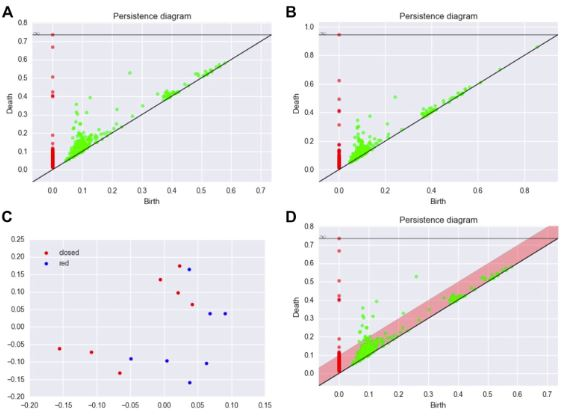
\includegraphics[width=0.85\linewidth]{./figures/Figura14.JPG}
    \caption{
        (A, B) Dos diagramas de persistencia para dos configuraciones de la MBP
        (Maltose-Binding Protein).
        (C) Configuraci\'on MDS (Multi-Dimensional Scaling)
        para la matriz de distancias de cuello de botella.
        (D) Diagrama de persistencia con regi\'on de confianza para la MBP.
    }
    \label{fig:Figura 14}
    \vspace{15pt}
\end{figure}